%! Author = ibw
%! Date = 09.11.23

% Preamble
\section{Evaluation}
\subsection{Erheben und Gewichten der Anforderungen}
\subsection{Exkurs Architektur}
\subsubsection{High Availability und Replikation}
Wenn eine Datenbank HA (High Availability), also Hochverfügbar, sein soll, braucht es eine Primäre und mindestens eine Sekundäre- oder \Gls{Failover}-Datenbank.
Um Datenverlust zu vermeiden, müssen die Daten permanent von der Primären auf die sekundäre Datenbank repliziert werden, dies nennt man Replikation\cite{D9RDXENY}.
Dabei wird zwischen den folgenden beiden Replikationen unterschieden:
\\\textbf{Synchrone Replikation}\\
Wenn bei einer Synchronen Replikation eine Transaktion abgesetzt wird, wird der Commit auf der primären Seite erst gesetzt, wenn die Änderung auf der sekundären Seite oder den sekundären Seiten ebenfalls eingetragen und Committed ist.
Bis zu diesem Moment ist die Transaktion nicht als Committed.

Dies wird dann zum Problem, wenn keine Verbindung mehr zu mindesten einer sekundären Seite vorhanden ist.
Zudem wird die Synchrone Replikation bei hohen Latenzen zum Bottleneck der Datenbank.

\textbf{Asynchrone Replikation}\\
Bei der Asynchronen Replikation wird eine Transaktion erst auf der eigenen primären Seite Committed und erst dann an die sekundären Nodes gesendet.
Besonders bei hohen Latenzen bleibt die Datenbank immer perfomant, allerdings kann es je nach Latenz und genereller Auslastung zu Datenverlusten kommen, wenn es zum \Gls{Failover} kommt.
\subsubsection{Quorum}
\label{chap:Quorum}
Ein Quorum-System

Hier ein Beispiel wie sie in den Artikeln \cite{UMIGLCCI, YDS7DTYM, V4XLXN7W}
\begin{description}
    \item \textbf{Quorum}\hfill \\Die Mehrheit der Server, die einen funktionierenden Betrieb gewährleisten können, ohne eine \Gls{Split-brain}Situation zu erzeugen.
    Die Formel ist gemeinhin \(n/2 + 1\)
    \item \textbf{Throughput}\hfill \\Beschreibt, wie sich die Anzahl Nodes auf die Schreibgeschwindigkeit der Commitments auf die restlichen Nodes auswirkt.\\Die verdopplung der Server halbiert i.d.R. den Throughput.
    \item \textbf{Fehlertoleranz}\hfill \\Beschreibt, wie viele Nodes ausfallen können, damit der Cluster noch Arbeitsfähig ist.\\Wobei eine erhöhung der Nodes von 3 auf 4 die Fehlertoleranz nicht erhöht da nun eine \Gls{Split-brain}-Situation entstehen kann.
\end{description}
%\begin{landscape}
%\begin{table}[]
%\resizebox{\columnwidth}{!}{%
%\begin{tabular}{@{}llll@{}}
%\toprule
%\textbf{Anzahl Nodes} & \textbf{Quorum} & \textbf{Fehlertoleranz} & \textbf{Representative Throughput} \\ \midrule
%1                     & 1               & 0                                               & 100                                \\
%2                     & 2               & 0                                               & 85                                 \\
%3                     & 2               & 1                                               & 82                                 \\
%4                     & 3               & 1                                               & 57                                 \\
%5                     & 3               & 2                                               & 48                                 \\
%6                     & 4               & 2                                               & 41                                 \\
%7                     & 4               & 3                                               & 36                                 \\ \bottomrule
%\end{tabular}%
%}
%\caption{Quorum Beispiele}
%\label{tab:quorum-beispiele}
%\end{table}
%\end{landscape}
%\subsubsection{Split-brain}
%\label{chap:Split-brain}
\begin{table}[]
\resizebox{\columnwidth}{!}{%
\begin{tabular}{@{}llll@{}}
\toprule
\textbf{Anzahl Nodes} & \textbf{Quorum} & \textbf{Fehlertoleranz} & \textbf{Representative Throughput} \\ \midrule
1                     & 1               & 0                       & 100                                \\
2                     & 2               & 0                       & 85                                 \\
3                     & 2               & 1                       & 82                                 \\
4                     & 3               & 1                       & 57                                 \\
5                     & 3               & 2                       & 48                                 \\
6                     & 4               & 2                       & 41                                 \\
7                     & 4               & 3                       & 36                                 \\ \bottomrule
\end{tabular}%
}
\caption{Quorum Beispiele}
\label{tab:quorum-beispiele}
\end{table}
\subsubsection{CAP Theorem}
Das CAP Theorem besagt, das nur zwei der drei folgenden drei Merkmale von verteilten Systeme gewährleistet werden können\cite{EE6EQHU2}.
\\\textbf{Konsistenz - Consistency}
Die Datenbank ist Konsistent, alle Clients seher gleichzeitig die gleichen Daten unabhängig auf welchem Node das Zugegriffen wird.
Hierzu muss eine Replikation der Daten an alle Nodes stattfinden und der Commit zurückgegeben werden, also eine Synchrone Replikation stattfinden.
\\\textbf{Verfügbarkeit - Availability}
\\\textbf{Ausfalltoleranz / Partitionstoleranz - Partition tolerance}

\Gls{PostgreSQL}, \Gls{Oracle Database}oder \Gls{IBM DB2}präferieren CA, also Konsistenz und Verfügbarkeit.
\subsubsection{Skalierung}
Datenbanken müssen skalierbar sein.
Dabei wird unterschieden zwischen einer vertikalen Skalierung (scale-up) und horizontaler Skalierung (scale-out).
Bei der vertikalen Skalierung werden den DB-Servern mehr CPU-Cores und Memory sowie zum Teil Storage hinzugefügt, wobei der Storage in jedem Fall wachsen wird.
Beim horizontalen Skalieren werden weitere DB-Nodes in den Cluster eingehängt\cite{IZSGZLVT}:
\begin{figure}[H]
    \centering
    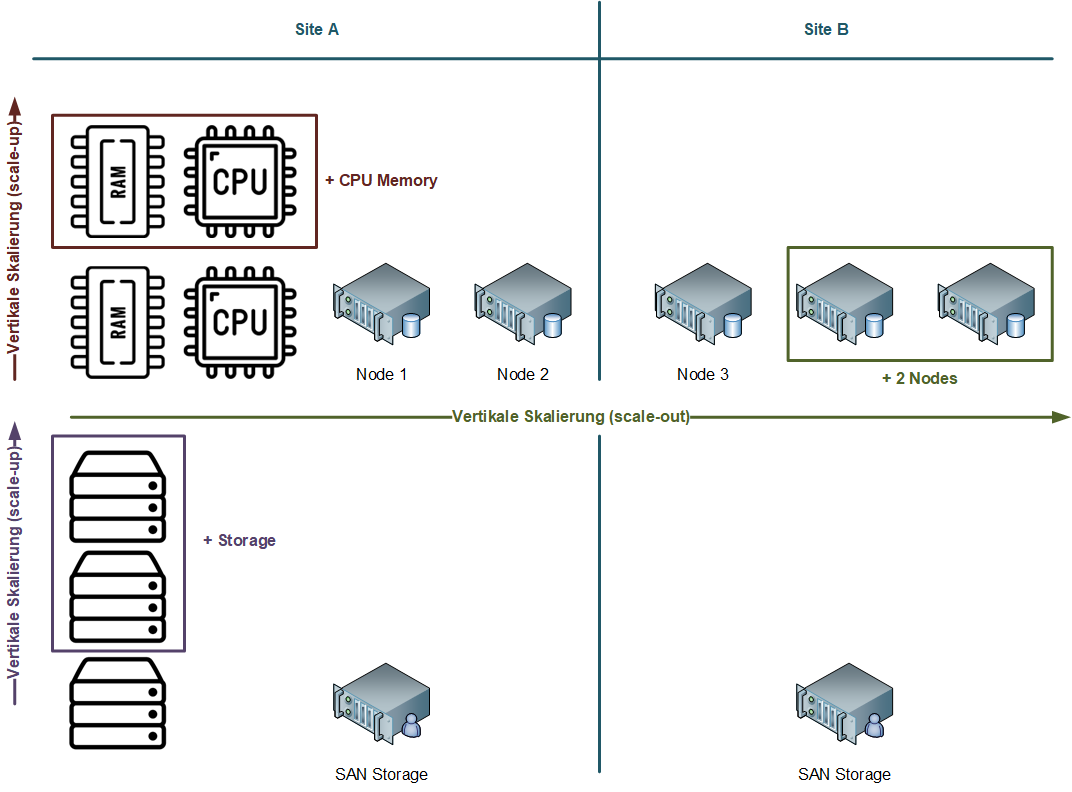
\includegraphics[width=1\linewidth]{source/implementation/evaluation/Skalierung}
    \caption{Datenbankskalierung}
    \label{fig:Datenbankskalierung}
\end{figure}

\subsection{Testziele erarbeiten}
\subsection{PostgreSQL Benchmarking}
PostgreSQL bietet ein Benchmarking-Tool,\cite{TYJFF7AB,VXNYQFTE} mit dem die DB Vermessen werden kann.
\subsection{Analyse gängiger PostgreSQL HA Cluster Lösungen}
\subsubsection{\Gls{PostgreSQL} Replikation}
PostgreSQL bietet von Haus aus Möglichkeiten, um Replikationen durchzuführen.
Dabei ist nicht jede gleich gut für jedes Szenario geeignet\cite{FZAHA89U}.

\subsubsection{KSGR Lösung}
Das Kantonsspital Graubünden hat basierend auf \gls{keepalived} wird geprüft ob die primäre Seite erreichbar und betriebsbereit ist.
Trifft dies nicht mehr zu, wird ein \Gls{Failover} durchgeführt\cite{NLF2IDBZ}.
Ist die primäre Seite wieder verfügbar, wird ein Restore auf die primäre Seite gefahren.

Es wird beim Restore immer ein komplettes Backup der sekundären Seite auf die primäre Seite übertragen.
Ursache ist, dass die normalerweise für den Datenrestore benötigten \Gls{PostgreSQL} Board mittel nur für eine relativ kurze Zeit eingesetzt werden können ehe die differenzen zwischen den beiden Seiten zu gross werden.

Bei kleinen Datenbanken wie jene für \Gls{Harbor} und \Gls{GitLab} ist die Zeit die hierfür benötigt wird, nicht relevant.
Sind die Datenbanken auf dem \Gls{PostgreSQL Cluster} jedoch grösser, kann der Restore mehrere Minuten dauern.
\subsubsection{pgpool-II}
pgpool-II ist eine Middleware die zwischen einem \Gls{PostgreSQL Cluster} und einem PostgreSQL Client gesetzt wird.
pgpoolII bietet folgende Funktionen\cite{EXVNLICT,3XWCD3KX}:
\textbf{High Availability}
pgpool-II bietet einen automatic \Gls{Failover} genannten Service an.
Dieser schwenkt auf einen Standby-Server und entfernt den Defekten Server.
Um false positive Events und Split-brains zu verhindern setzt pgpool-II auf einen eigens entwickelten \Gls{Quorum}-Algorithmus.
\\\textbf{Connection Pooling}
\\\textbf{Replikation}
\\\textbf{Load Balancing}
Ähnlich wie Oracle Active Data Guard \cite{6294443C} bietet auch pgpool-II die Möglichkeit, SELECT-Queries und Backup-Jobs auf die Secondary-Nodes umzuleiten um den Primary Node zu entlasten.
\\\textbf{Limiting Exceeding Connections}
\\\textbf{Watchdog}
\\\textbf{In Memory Query Caching}

\subsubsection{pg\_auto\_failover}
\subsubsection{Patroni}
\subsubsection{CloudNativePG}
\subsection{Installation verschiedener Lösungen}
\subsection{Gegenüberstellung der Lösungen}
\subsection{Entscheid}